\documentclass{article}

\usepackage{pdfpages}
\usepackage{graphicx}

\graphicspath{ {./images/} }

\title{
    \vspace{-4.0cm}
    {\Huge Social Routing}\\[0.5cm]    
    \textsc{\Large Project and Seminar}\\[0.5cm]
    \textsc{\large Instituto Superior de Engenharia de Lisboa}\\[0.5cm]
}

\date{\today}
\author{   
    \begin{minipage}{0.4\textwidth}
        \begin{flushleft} \large
        \emph{Authors:}\\
        Baltasar Brito\\
        {\small email: baltasar.brito@gmail.com}\\
        {\small phone: 915953552}\\
        Bernardo Costa\\
        {\small email: bjmcosta97@gmail.com}\\
        {\small phone: 913897555}\\
        \end{flushleft}
    \end{minipage}
    ~
    \begin{minipage}{0.4\textwidth}
        \begin{flushright} \large
        \emph{Supervisor:} \\ 
        Pedro Félix\\
        {\small email: pedrofelix@cc.isel.ipl.pt}\\  
        \end{flushright}
    \end{minipage}\\[2cm]  
}

\begin{document}     
    
    \maketitle
 
    \section{Introduction} 

        The project consists of a system that provides the ability to define and share touristic pedestrian routes. It allows
        area exploration by using user made routes as virtual tour guides to other users. It has the following functionalities:
        \begin{itemize}
            \item Route creation.
            \item Ability to search routes.
            \item Route live tracking.
            \item Route updates.
            \item Route characterization.
        \end{itemize}

    \newpage
    

    \section{Analysis}

        \subsection{Use case}
            In the context of the application, a route is a path from point A to point B, that goes through user selected sub paths
            that might either have relevance or simply provide the fastest way to the next point of interest of that route. 

            An example of events when using the application might be:

            A user at his hotel decides he wants to go sightseeing for an hour and check the surrounding area by foot.
        
        \begin{itemize}  
            \item The user starts the application and searches for a route inserting his location and time available to spend on a route.
            \item The application suggests the top 3 routes available according to proximity to the user starting point, route evaluation and time necessary to complete the given route. 
            \item The user selects the route and is shown the directions in real time on a map that he has to follow to undergo such route until it is done.
            \item The user finishes the route and evaluates it, with the possibility of adding a suggestion to it. 
        \end{itemize}
        
        \subsection{Challenges}
            
            Considering the geolocation focused nature of the project there are some challenges to overcome:

            \begin{itemize}
                \item Characterization of a route: the metadata of a route which may contain elements such as travel time, ground elevation, ground type, age range, category, best time of day to transverse.
                \item Route creation, storage and visual representation: on the front-end side, how a route is represented and its creation made available to a user and on the back-end side the way that the information regarding the route is saved.
                \item Route searching: given search parameters it should be presented to the user the best possible route for his personal case.  
                \item User authentication: using an external service.
                \item Live tracking: using an external service, the user must be able to follow the route in real time.
                \item Path to the route and its ordering: given a starting location, a path to the beginning of a route must be generated, taking the route's ordering into consideration.
                \item External APIs comprehension and usage.
            \end{itemize}

    \section{System Structure}
        The project will be developed in three major components communicating with each other, separating concerns and business logic.
        
        \begin{figure}[h]            
            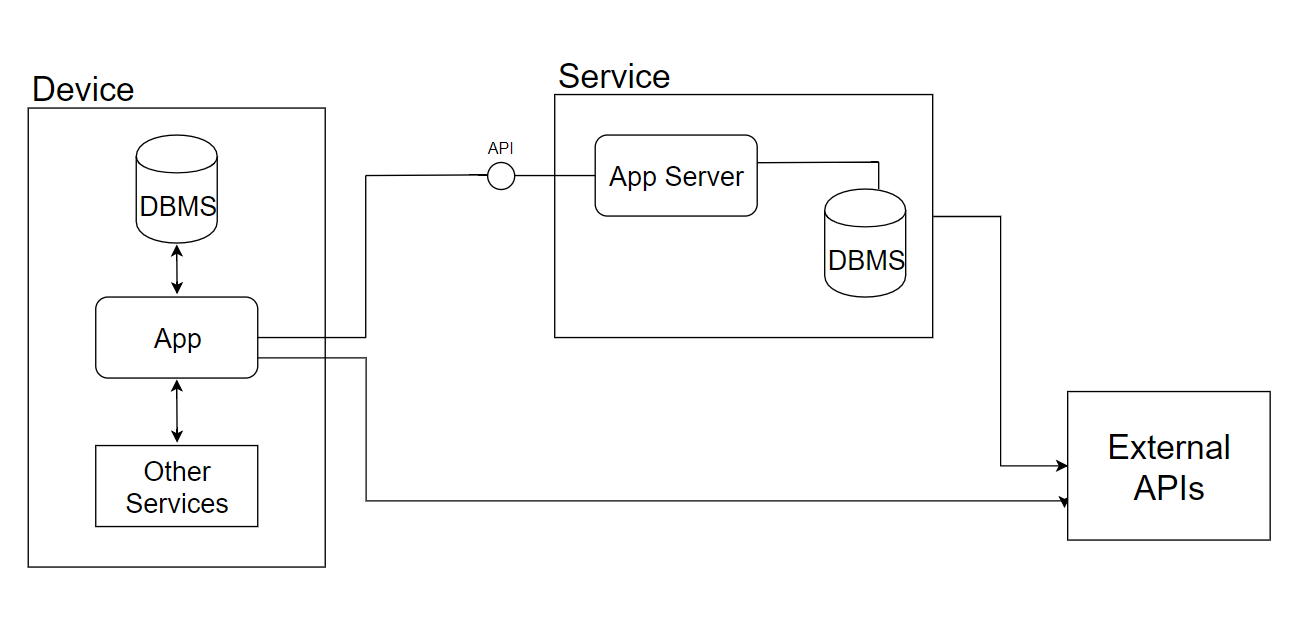
\includegraphics[width=\textwidth]{images/project-structure/system-structure.PNG}
        \end{figure}  

        \subsection{Device}  
            The project will have a mobile component which consists of an Android application. 
            This is the component that a user will interact with and is dependent of other internal and external services.
        \subsection{Social Routing Service}
            The system database and server are located in this component and together they hold the business logic of the system.
            This logic is exposed to the outside components through an API.
        \subsection{External APIs}
            This component encompasses the external elements of the system, already created by a third party, to provide a faster project development
            and to allow functionality extension instead of functionality recreation. 
    \section{Timeline}   

\end{document}